\section{Deep Learning Models}
\label{chap:dl-models}

This chapter presents the key components for developing and evaluating deep learning models.
This includes both the selection of suitable models and the criteria for assessing their performance.

For this work, Keras version 3.10.0 was used as a high-level API for modeling and training neural networks \cite{keras-home}.
Instead of the standard TensorFlow backend, PyTorch version 2.7.1 was used as the backend.
A key reason for this decision was its better support on Windows, compared to TensorFlow \cite{tf-windows}, particularly with regard to installation and compatibility with existing CUDA drivers.
By using Keras in combination with the PyTorch backend, user-friendly modeling could be combined with stable and well-supported execution on Windows systems.

%TODO: Es werden Regressions und Klassifikationsmodelle trainiert

The model architectures used in this work are not based on specific, citable publications, but were designed as part of an experimental and iterative development process.
The goal was to construct powerful models well-suited to the given problem.
Particularly with regard to processing sequential data of limited length and high variability.

Established neural building blocks such as 1D convolutional layers, GRUs, attention mechanisms, and transformer components were used, the fundamentals of which are comprehensively documented in the literature.
However, the specific design of the model architectures, such as the combination of multiple parallel CNN paths, the integration of GRUs after convolution steps, or the use of Global Average Pooling instead of flattening, represents a creative and pragmatic composition of its own.

Additionally, all models were automatedly optimized using Optuna, so that architectural decisions were also influenced by the hyperparameter search.
In many cases, initial ideas originate from non-scientific sources such as blog posts, online tutorials, or community code snippets, which are not scientifically citable.

In summary, the developed models are original variations, inspired by familiar architectural elements, but not directly adopted or reconstructed from specific publications.
This allows for greater flexibility and reinforces the experimental nature of the work.

For both regression and classification models, 13 different architectures were used, which can be divided into neural networks, convolutional neural networks, long short-term memories, and transformers.

\subsection{Metrics}

% TODO

\subsection{Optuna}

In modern machine learning methods, the selection of hyperparameters plays a central role in model performance.
Hyperparameters such as learning rate, the number of layers in a neural network, or regularization strengths directly influence the behavior and generalization of the model.
The search for optimal values for these parameters, the so-called hyperparameter optimization, is often a time-consuming and computationally intensive process \cite{hyperparameter-importance}.

Optuna is a modern framework for automated hyperparameter optimization designed for efficiency, flexibility, and ease of use.
It was developed to enable easy integration into existing machine learning pipelines while providing powerful, goal-oriented optimization.

The goal of Optuna is to automatically find those hyperparameter combinations that satisfy a specific optimization criterion (e.g., minimum validation error rate or maximum accuracy).
The search process should be as efficient as possible, requiring as few model training sessions as possible \cite{optuna-hyperparameters}.

In this work, Optuna was used to automatically run multiple training models with different hyperparameters to find the best hyperparameters.
In the relevant sections of the next chapters, the range of the hyperparameters for each model will be mentioned.

\subsection{Neural Networks}
\label{chap:nn}

Neural networks are among the central methods of machine learning and form the basis of many modern deep learning models.
The simplest and most widely used form is the feedforward neural network (FNN), also known as a multilayer perceptron (MLP).
Such networks are universally applicable and, with appropriate structuring, can be used for classification, regression, and pattern recognition.

A classic neural network consists of several layers of artificial neurons that forward information in a fixed order from input to output.
The structure can be divided as follows \cite{nn-basics}:

\begin{enumerate}
    \item \textbf{Input Layer:} Accepts the raw input data, e.g., a vector form of a time series or preprocessed features.
    \item \textbf{Hidden Layers:} One or more layers of artificial neurons, each of which calculates a weighted sum of the inputs and further processes it using an activation function.
    Typical activation functions are ReLU, sigmoid, or tanh.
    \item \textbf{Output Layer:} Provides the final result, e.g., class membership (for classification) or continuous value (for regression).
\end{enumerate}

In this work, three different neural network models have been tested.
The tested models are different in their complexity, depth, and methodical approach to data processing.

\subsubsection{Base Model with Flatten-Architecture}

The first model follows a classic feedforward approach, with one to three dense layers, each with 32 to 128 neurons and a rectified linear unit (ReLU) activation function.
The ReLU activation function was used because it provides an efficient calculation and a good gradient propagation with fewer vanishing gradients \cite{springer-ml-basics}.
Either before or after the dense layers, the input data are flattened \cite{keras-flatten}.
This decision influences whether the model processes all timepoints as a vector early on or treats each time step separately.
This architecture was used as a simple baseline model to obtain a quick training and a first baseline model.

The learning rate of the Adam optimizer ranges between $10^{-5}$ and $10^{-2}$, while the input layer has a length of 5 to 150
All hyperparameters are managed by Optuna.

\lstinputlisting[language=Python, caption=Base FNN, label=lst:base-model, style=python]{python/models/nn_base.py}

\subsubsection{Dropout Neural Network}

In the second model, the data is first converted into a one-dimensional vector using a flatten layer.
This is followed by one to three dense layers using ReLu activation.
Batch normalization supports stable and rapid convergence \cite{batch-normalization}, while dropout between 5\% and 35\% of the data is used as a regularization method to prevent overfitting \cite{keras-dropout}.
All other parameters are identical to those in the simple neural network.

The parameters tuned via Optuna control the model depth, the number of nodes per layer, the training dynamics, and the number of historical time points used as input.

\lstinputlisting[language=Python, caption=Dropout NN, label=lst:dropout-nn, style=python]{python/models/nn_dropout.py}

\subsubsection{Residual Neural Network}

The third model integrates a residual concept, originally known from image processing but also increasingly used in time series contexts.
The architecture consists of a linear shortcut branch connected to the main path via an additive connection \cite{residual-nn}.
This construction facilitates the training of deeper networks by improving gradient flow and preventing information loss through multiple layers.

In addition to the previous parameters, two additional variables controlled by Optuna are added: \verb|num_units_res_prep| and \verb|num_units_res|.
These determine the complexity of the residual branch.
The distinction whether flattening is done before or after the hidden layers is also included here to flexibly adapt data processing to the underlying data structure.

This architecture is particularly suitable for nonlinear and complex relationships, such as those frequently encountered in ETH price forecasting.
The residual path allows the model to pass on basic information directly, while deeper layers learn abstract features.

\lstinputlisting[language=Python, caption=Residual NN, label=lst:residual-nn, style=python]{python/models/nn_residual.py}

\subsection{Long Short-Term Memory Models}
\label{chap:lstm}

In addition to traditional dense neural networks, recurrent neural networks (RNNs) based on the Long Short-Term Memory (LSTM) architecture were also used.
LSTMs are specifically designed to capture temporal dependencies in sequential data and retain long-term information across multiple time steps \cite{lstm-usage}.
This is particularly important for financial data such as ETH prices, as current prices are often influenced by past developments.

LSTM cells have an internal memory structure and three control mechanisms (input, forget, and output gates) that allow the network to decide which information should be stored, overwritten, or passed on \cite{lstm-cell}.
This effectively mitigates the so-called vanishing gradient problem of traditional RNNs \cite{lstm-gradient-problem}.

\subsubsection{Base LSTM}

This model consists of one or two stacked LSTM layers followed by a dense output layer.
If only one LSTM layer is added, it returns the result directly.
With multiple layers, the temporal sequence information is passed to the second LSTM layer.

Similar to feedforward neural networks, the number of layers, the number of neurons per layer, the learning rate, and the length of the input window used are managed via Optuna.

This model represents the basic form of a sequential predictor and is well suited for simple time series patterns.

\lstinputlisting[language=Python, caption=Base LSTM, label=lst:base-lstm, style=python]{python/models/lstm.py}

\subsubsection{Dropout LSTM}

This variant extends the standard model with dropout layers inserted between the LSTM units, discarding between 5\% and 50\% of the data.

The additional parameter is also determined by Optuna and allows fine-tuned control over the regularization strength.
This model is particularly useful when working with noisy or volatile price trends, such as cryptocurrencies.

\lstinputlisting[language=Python, caption=Dropout LSTM, label=lst:dropout-lstm, style=python]{python/models/lstm_dropout.py}

\subsubsection{Bidirectional LSTM (BiLSTM)}

The third model uses bidirectional LSTM layers.
These process the input sequence forward and backward simultaneously, allowing both earlier and later information to be incorporated into the internal state \cite{bi-lstm}.

This architecture can be particularly valuable in the context of ETH predictions based on historical data, as it allows for better detection of symmetric patterns or turning points in price trends.

The hyperparameter structure is similar to the previous models, but the modeling is performed using double LSTM paths.

\lstinputlisting[language=Python, caption=Bidirectional LSTM, label=lst:bi-lstm, style=python]{python/models/lstm_bi.py}

\subsubsection{Encode-Decode Model with Repeat-Vector}

The fourth model is based on an encoder-decoder approach, as used in machine translation.
The input sequence is first converted into a fixed context vector by an LSTM layer, which is then duplicated multiple times using RepeatVector \cite{keras-repeat-vector}.
A decoder-LSTM interprets this vector sequentially to generate a temporally structured output.

This architecture is particularly suitable for multistep forecasting, as it can map not only the next value but an entire sequence of future values.
The final preprocessing is performed using \verb|TimeDistributed(Dense(...))| to calculate a separate output for each time step \cite{keras-time-distributed}.

\lstinputlisting[language=Python, caption=Encode-Decode LSTM, label=lst:encode-decode-lstm, style=python]{python/models/lstm_encode_decode.py}

\subsection{Convolutional Neural Networks}
\label{chap:cnn}

Convolutional neural networks (CNNs) represent a special architecture within deep learning that was developed specifically to process data with spatial structures, such as images.
Compared to traditional feedforward networks, CNNs are significantly more efficient in handling high-dimensional inputs and have established themselves as standard methods in numerous application areas such as object detection, natural language processing, and time series analysis \cite{cnn-for-time-series}.

The key difference between CNNs and classical neural networks lies in the use of so-called convolutional layers, which exploit the local structures in the input data.
Instead of connecting every neuron to all input values (as with a fully connected layer), local filters (kernels) are used that respond only to a small portion of the input space.
These filters are automatically learned during the training process \cite{cnn-for-time-series}.

Time series typically exhibit temporal dependencies, repetitions, seasonal patterns, or short-term fluctuations.
Classic methods for processing this data, such as LSTM networks, explicitly model such dependencies using recursive states.
CNNs, on the other hand, uses an alternative approach, called local convolutions, which also serve time series to detect relevant patterns or changes over short or medium periods of time \cite{cnn-local-convolution}.

The advantages of using CNNs for time series include:

\begin{enumerate}
    \item \textbf{Parallel Processing:} CNN does not require recursive loops, e.g., compared to LSTMs.
    \item \textbf{Local Pattern Detection:} CNNs can detect local patterns, such as peaks, fluctuations, or trend changes.
    \item \textbf{Computational Complexity:} CNNs requires lower computational power compared to recursive architectures.
\end{enumerate}

\subsubsection{Base CNN}

The simplest variant consists of two stacked one-dimensional convolutional layers, followed by maxpooling, and two dense layers for output preparation.
The position of the flattening layer affects the processing order between the dense and the sequence structure.

The hyperparameters tuned by Optuna are the number of units in the convolutional layers, the length of the filters (Kernel size), the size of the maxpooling region, the position of the flattening layer, and the number of neurons in the dense layers.

\lstinputlisting[language=Python, caption=Base CNN, label=lst:simple-cnn, style=python]{python/models/cnn_simple.py}

\subsubsection{Deep CNN}

The model shown here represents an extension of a simple CNN model (Base CNN).
While the simple model uses only a single 1D convolutional layer followed by a pooling and dense layer, this Deep CNN model uses two consecutive Conv1D layers.
This additional depth allows the network to learn more complex and hierarchical feature representations from the input data \cite{cnn-deep-more-complex}.
This is particularly useful for timeseries with multi-level dependencies or subtle patterns.
The model is complemented by a MaxPooling layer, which reduces the temporal resolution and counteracts overfitting.
The optional placement of the Flatten layer allows for the evaluation of different configurations of feature identification, which in turn increases model flexibility.
Overall, this more deeply structured CNN enables more powerful modeling than the flattened variant.

\lstinputlisting[language=Python, caption=Deep CNN, label=lst:deep-cnn, style=python]{python/models/cnn_deep.py}

\subsubsection{Attention CNN}

An alternative architecture uses multiple parallel convolutional layers with different kernel sizes.
This allows the model to detect both short-term and medium-term patterns simultaneously.
The resulting feature maps are combined using an attention layer to highlight important sequence segments \cite{cnn-attention}.

This is followed by global average pooling and a dense layer for output generation.

\lstinputlisting[language=Python, caption=Attention CNN, label=lst:attention-cnn, style=python]{python/models/cnn_attention.py}

\subsubsection{Concatenation CNN}

A slightly modified version replaces the attention module with a simple concatenation of the feature maps.
This allows the model to pass the extracted features directly without performing weighting \cite{keras-concat}.

This variant is computationally less expensive than the attention-based one and is well-suited when all filter outputs should be treated equally.

\lstinputlisting[language=Python, caption=Concatenation CNN, label=lst:multiscale-cnn, style=python]{python/models/cnn_multi_scale.py}

\subsubsection{CNN-GRU Hybrid Model}

The Gated Recurrent Unit (GRU) model is a simplified variant of the LSTM and was developed to reduce computational effort and model complexity.
Compared to LSTM, GRU has only two gates, an update gate and a reset gate, instead of three (input, forget, and output gates in LSTM).
This makes GRU faster to train, requires less memory, and delivers comparable results in many tasks \cite{gru-basics}.

To combine the advantages of both architectures, a hybrid CNN-GRU model was also implemented.
A Conv1D layer first extracts local features from the sequence, which are then sequentially processed using a GRU module to capture long-term dependencies and trends \cite{cnn-gru}.

This model is particularly well-suited for linking local patterns (using CNN) with temporal dependencies (using GRU).
The final dense layers perform the transformation to the target variable as usual.

\lstinputlisting[language=Python, caption=CNN + GRU, label=lst:gru-cnn, style=python]{python/models/cnn_gru.py}

\subsection{Regression Models}
\label{chap:regression-models}

Regression models were used to predict the next 30 minutes of logarithmic returns as a continuous sequence.
For this purpose, all models mentioned in \autoref{chap:nn}, \autoref{chap:lstm}, and \autoref{chap:cnn} were trained on the training data (\autoref{tbl:train-data}) for 20 trials of Optuna with 30 epochs each.
After each epoch, the model was evaluated using the validation data (\autoref{tbl:validation-data}).
To achieve a continuous sequence as output, the activation function in the last dense layer of the above-mentioned models was set to \verb|linear| and the number of neurons to 30.

\subsubsection{Loss-Function}
\label{chap:regression-loss}

In order to incorporate the trading context during model training and evaluation, traditional loss functions such as the root mean squared error have been avoided.
Instead, a proprietary loss function was implemented that calculates realized profit and loss.
The value of the loss function decreases the more profit is generated.

As mentioned above, the output of the regression models are either a sequence of the next expected logarithmic returns by minute.
The first step of the loss function is to decide whether the opened position should be a long or short position.
This is decided by cumulating the predictions.
The absolute maximum is then determined for the cumulative values greater than and less than zero.
If the absolute maximum of the values greater than zero is greater than the absolute maximum of the values less than zero, a long position is opened.
Otherwise, a short position is opened.
\autoref{fig:loss-long-position-decision} illustrates the decision using a long position as an example.

\begin{figure}[H]
    \centering
    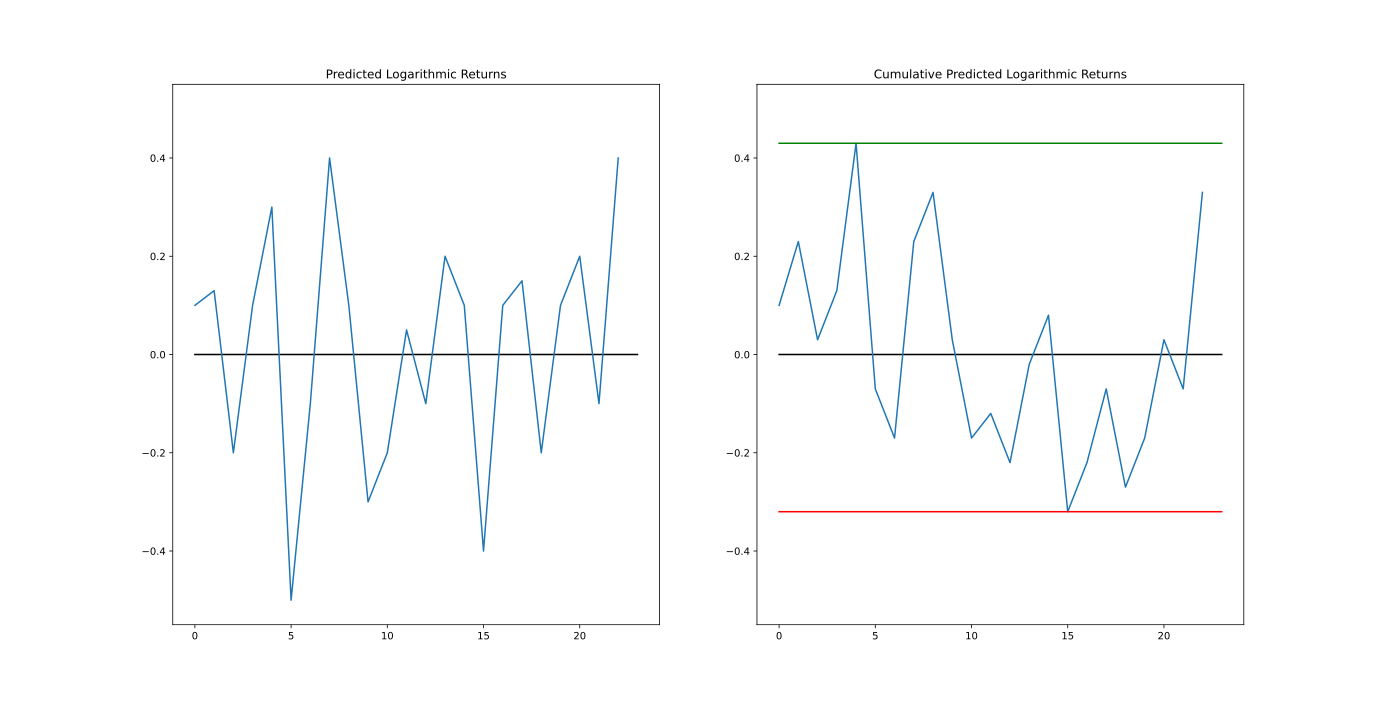
\includegraphics[width=\textwidth]{images/models/loss_direction}
    \caption{Long Position Decision}
    \label{fig:loss-long-position-decision}
\end{figure}

After the direction decision, the stop-loss and take-profit levels must be determined.
For long and short positions, there are two possibilities at which specific level the stop-loss and take-profit are set, based on the global high and low of the cumulative predicted logarithmic returns.
If a long position was previously decided and the global high comes after the global low, the stop-loss is set at the global low and the take-profit at the global high.
However, if the global high comes before the global low, the stop-loss is set at the lowest low before the global high.
For short positions, the decision is exactly the opposite.

\autoref{fig:loss-tp-sl} shows the stop-loss and take-profit levels for all four cases.
The red areas mark the predicted unprofitable zones and the green areas mark the predicted profitable zones.

\begin{figure}[H]
    \centering
    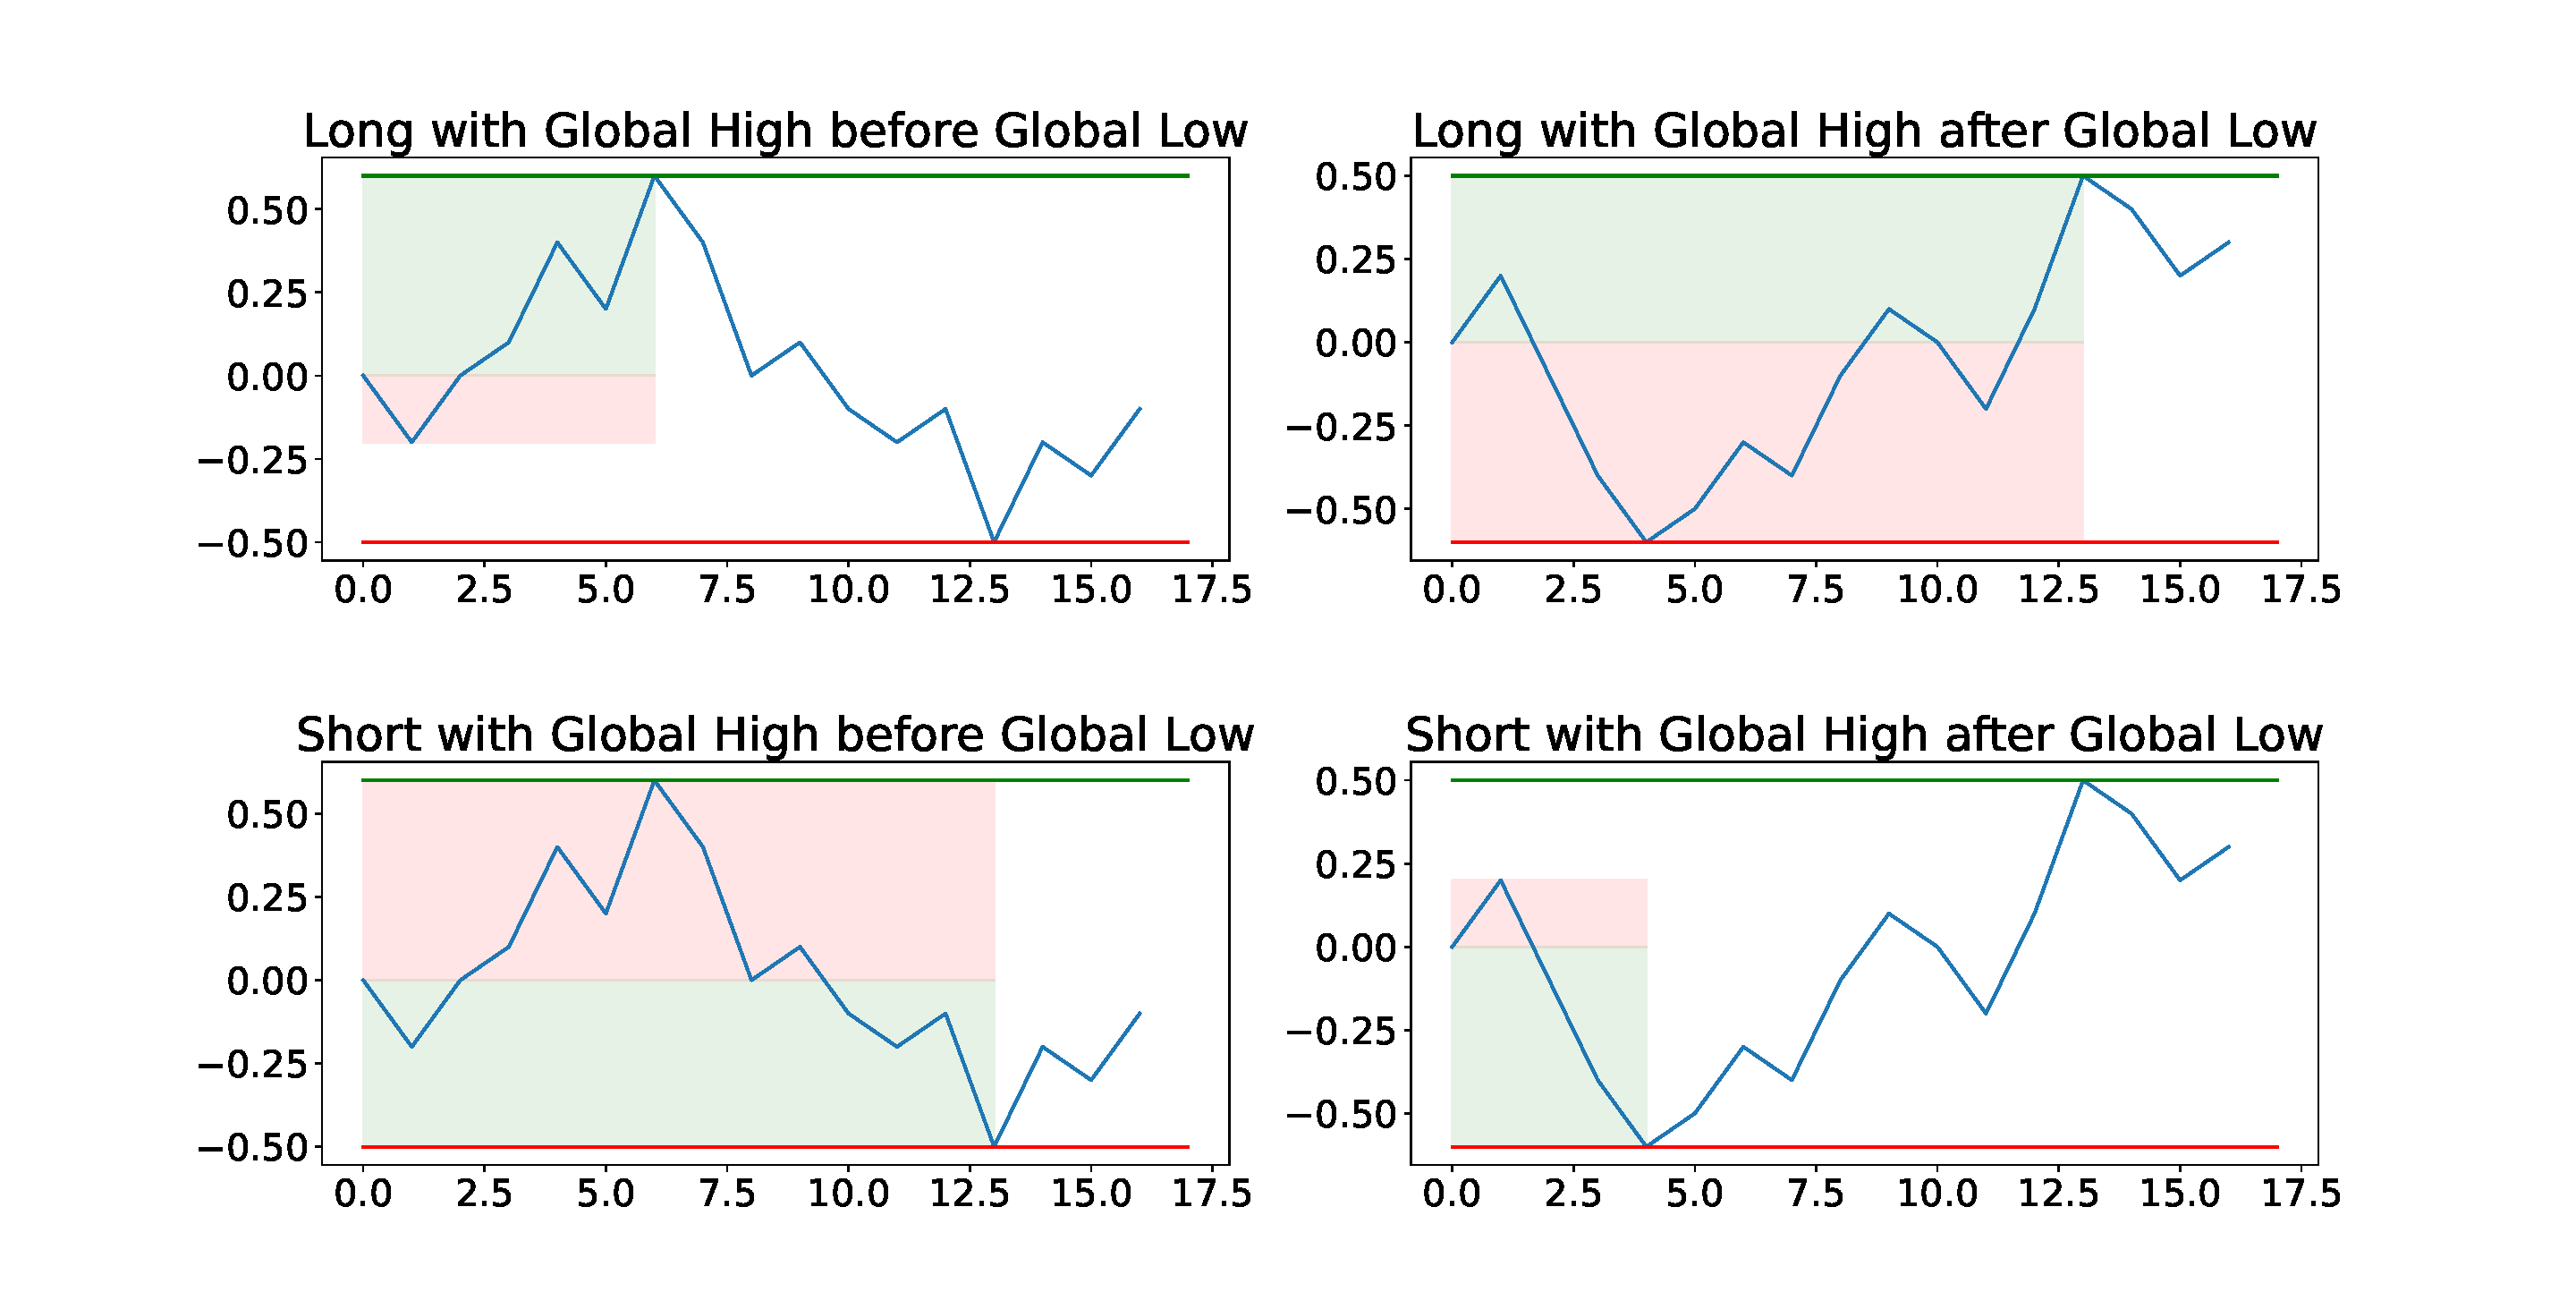
\includegraphics[width=\textwidth]{images/models/loss_tp_sl}
    \caption{Long Position Decision}
    \label{fig:loss-tp-sl}
\end{figure}

After the stop-loss and take-profit levels are determined, the actual logarithmic returns are used to calculate the profit or loss for each position.
If neither the stop-loss nor the take-profit is reached, the profit calculation defaults to the profit if the stop-loss is reached to ensure that the model predicts the correct take-profit more often.

\subsubsection{Model Evaluation}

%TODO

\subsection{Classification-Models}
\label{chap:classification-models}

Classification models were used to predict an action to be performed.
The action can be either buy, sell, or do nothing.
For that, the model predicts a probability for each of the three classes.
As with the \hyperref[chap:regression-models]{regression models}, the same models are used, but this time the last dense layer has only three neurons and the activation function \verb|softmax|.
The identical training and validation period was also used, and the training took place over 20 Optuna trials with 30 epochs each.

\subsubsection{Loss-Function}

For classification models, the categorical cross-entropy loss function was used.
This choice is common and well-suited for classification problems where the model output represents a probability distribution across multiple classes.
Mathematically, it is defined as follows:

\[
    L_{CCE} = -\sum_{i=1}^{C} y_i*log(\hat{y_i})
\]

Where $C$ denotes the number of classes, $y_i$ the actual value (usually encoded as a one-hot vector), and $\hat{y_i}$ the probability predicted by the model for class $i$.
This function penalizes the model particularly severely if it assigns a high probability to an incorrect class and rewards correct predictions with high confidence.

Categorical cross-entropy measures the difference between the actual target distribution and the probability distribution predicted by the model \cite{springer-ml-basics}.

\subsubsection{Model Evaluation}

%TODO